\documentclass[journal]{IEEEtran}

\usepackage{blindtext}
\usepackage{cite}
\usepackage{graphicx}
\usepackage{array}
\usepackage{color}
\usepackage{tabularx}
\usepackage{epsfig}
\usepackage{amsmath}
\usepackage{amssymb}
\usepackage{bm}
\usepackage{wasysym}
\usepackage{circuitikz}
\usepackage{float}
\usepackage{algorithm}
\usepackage{algorithmic}

\usetikzlibrary{arrows,shapes,calc,positioning}

\newcommand{\myscope}[2]
{\draw[thick,rotate=#2] (#1) circle (12pt)
(#1) ++(-0.35,-0.1) --++ (0.3,0.3) --++ (0,-0.3) --++(0.3,0.3) --++(0,-0.3);}

\begin{document}

\title{CSCE 221 \\ Problem Set 17}

\author{Jacob~Purcell,~\IEEEmember{Texas~A\&M,~Student}}

\maketitle
\section{}

The results of actual shortest path(left of graph) and Dijkstra's Algorithm(right of graph) are shown in Fig. 1. 
As one can see, the actual shortest path was overwritten with the addition of a negative value.

\begin{figure}[h!]
    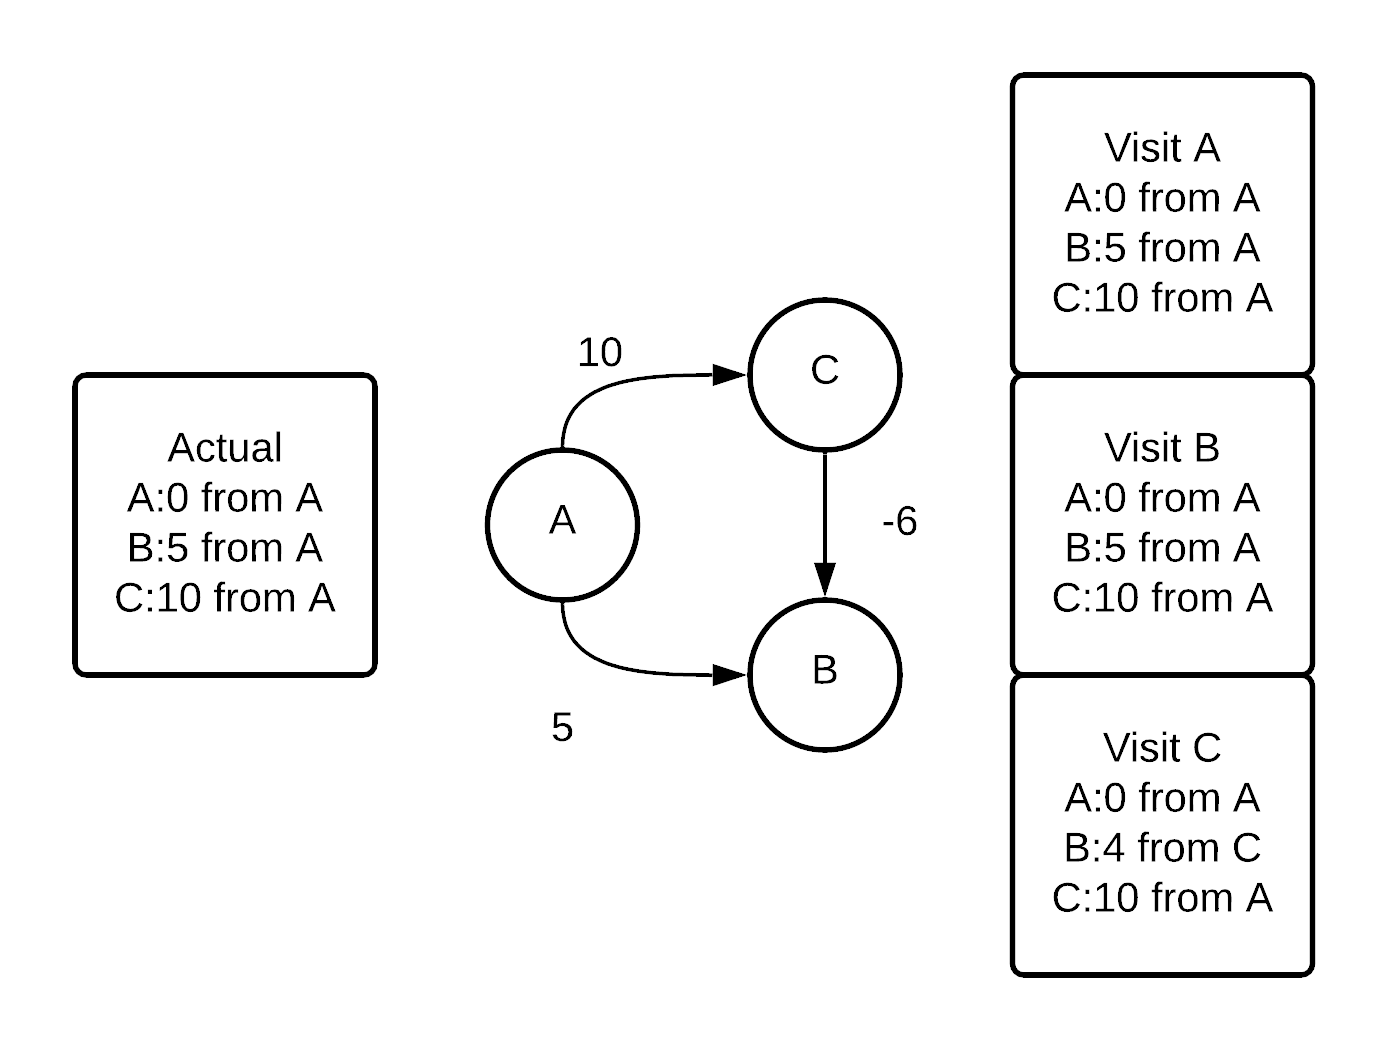
\includegraphics[scale = 0.17]{dnw.png}
    \caption{Dijkstra's Algorithm on graph with negative weight.}
\end{figure}

\section{}
\subsection{}
The count of number of shortest paths from one node to another can be accomplished by comparing every unchecked edge to the currnet minimum.
If the path being calculated is the same distance as the current minimum, increment the count. If the minimum is replaced, the count is reset.

\subsection{}
One can keep a number of edges from the origin node stored as a data variable. The shortest path is only updated if the current path is shorter or
the current path is the same distance but requires less edges.
\end{document}
